% DIOS, TEN MISERICORDIA DE NOSOTROS
% Jorwin
\subsection{Modelo matemático}
El sistema a analizar es el siguiente:
\begin{figure}[ht]
    \centering
    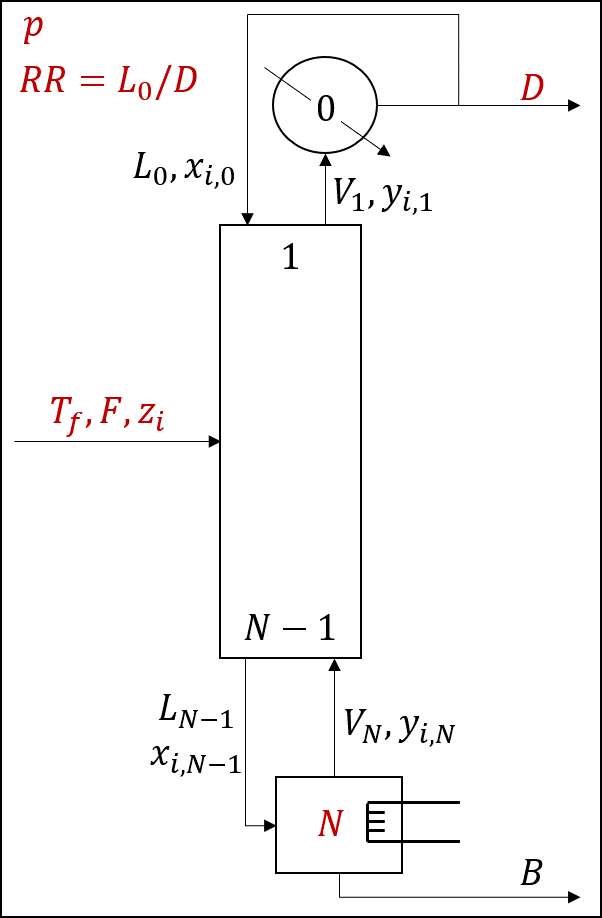
\includegraphics[width=0.7\linewidth]{../resources/flowcharts/diagrama_columna.png}
    \caption{Diagrama de una columna de destilación multicomponente}
\end{figure}

\newpage
\subsubsection{Suposiciones fundamentales}
Para elaborar un modelo matemático que pueda explicar y predecir el sistema es importante considerar las siguientes suposiciones:
\begin{enumerate}
    \item \textbf{Operación en estado estacionario:}\\
          Se asume que la columna opera de forma estacionaria, es decir, que las variables no cambian en el tiempo.
    \item \textbf{Equilibrio de fases en cada plato:}\\
          Se asume que el equilibrio de fases se alcanza en cada plato de la columna, por ende, las composiciones de las fases son iguales a las del equilibrio.
    \item \textbf{Mezcla ideal:}\\
          Se asume que la mezcla de componentes en la columna se comporta como una mezcla ideal, lo que implica que las propiedades termodinámicas de la mezcla se pueden calcular a partir de las propiedades de los componentes individuales.
    \item \textbf{Razón de reflujo constante:}\\
          Se asume que la razón de reflujo es constante a lo largo de la columna, lo que significa que la cantidad de líquido que se recicla al condensador es constante.
    \item \textbf{Columna adiabática:}\\
          Se asume que no hay transferencia de calor entre la columna y el entorno, lo que implica que la columna opera adiabáticamente.
\end{enumerate}

% Edson
\newpage
\subsubsection{Relaciones de equilibrio líquido-vapor}
El equilibrio líquido-vapor se refiere a que en cada plato, la tasa de evaporación será igual a la tasa de condensación para todos los compuestos. De no haber un equilibrio líquido-vapor, todo el líquido se evaporaría o todo el vapor se condensaría, de esta manera no se cumpliría el objetivo de fraccionar los gases ligeros del petróleo \parencite{subsec5_5ref3}.

El comportamiento de equilibrio para cada componente en cada plato se explica utilizando la constante de equilibrio $K_{i,j}$:
$$
    y_{i,j} = K_{i,j}(T_j, P_j)\ x_{i,j},
$$

donde:
\begin{itemize}
    \item $y_{i,j}$ es la fracción molar en la fase vapor.
    \item $x_{i,j}$ es la fracción molar en la fase líquida.
    \item $K_{i,j}(T_j, P_j)$ es la constante de equilibrio.
\end{itemize}

Para determinar la constante $K_{i,j}$ se utiliza la ecuación empirica de DePriester:
$$
    \ln{K_{i,j}} = \frac{a_1}{T^2} + \frac{a_2}{T} + a_3 + b_1 \ln(P) + \frac{b_2}{P^2} + \frac{b_3}{P},
$$

donde:
\begin{itemize}
    \item $a_1, a_2, a_3, b_1, b_2, b_3$ son constantes.
    \item $T_j$ es la temperatura del plato.
    \item $P_j$ es la presión del plato.
\end{itemize}

La expresión de $x_{i,j}$ es la siguiente:
$$
    x_{i,j} = \frac{l_{i,j}}{L_{j}},
$$

donde:
\begin{itemize}
    \item $l_{i,j}$ es la corriente molar del componente $i$ en el plato $j$.
    \item $L_j$ es la corriente molar del plato $j$.
\end{itemize}

% Jorwin
\newpage
\subsubsection{Temperatura de punto de burbuja}\label{ss_sec:temperatura_punto_burbuja}
El ``punto de burbuja'' de una mezcla es la temperatura (a una presión dada) a la que la mezcla líquida comienza a generar la primera burbuja de vapor, es decir, en la que se inicia la vaporización.

Para hallar la temperatura de punto de burbuja se requiere conocer la presión de operación inicial de la columna y las fracciones molares líquidas en el destilado y el residuo. Después se calcula la constante de equilibrio para cada componente utilizando la ecuación de DePriester.

A continuación, se obtienen las fracciones molares de vapor utilizando:
$$
    y_{i,j} = K_{i,j} x_{i,j}
$$

Finalmente, se verifica que la suma de las fracciones molares de vapor cumpla:
$$
    \sum_i y_{i,j} = 1
$$

Este procedimiento es iterativo. Si la suma resulta mayor a 1, se debe disminuir la temperatura propuesta; si es menor, se aumenta. El proceso se repite hasta que se cumpla la igualdad, determinándose así la temperatura de punto de burbuja.

% Jorwin
\newpage
\subsubsection{Número de platos reales y plato alimentado}\label{ss_sec:platos_equilibrio_alimentacion}
Para determinar el número de platos reales y el punto alimentado en una columna de destilación, se emplea el método de Fenske-Underwood-Gilliland-Kirkbride. Este método introduce los conceptos de componente ligero ($lk$) y componente pesado ($hk$), definidos respectivamente como aquellos que se concentran en el destilado y en el residuo.

A continuación, se describen de manera sistemática los pasos a seguir:
\begin{enumerate}
    \item \textbf{Balance de masa en el destilado y el residuo:}\\
          Se parte de las siguientes relaciones:
          $$
              f_{lk} = \frac{D_{lk}}{F_{lk}} \quad \longrightarrow \quad D_{lk} = f_{lk} F_{lk} z_{lk},
          $$
          $$
              f_{hk} = \frac{D_{hk}}{F_{hk}} \quad \longrightarrow \quad D_{hk} = f_{hk} F_{hk} z_{hk},
          $$

          donde $ D_{lk} $ y $ D_{hk} $ representan las corrientes molares de los componentes ligero y pesado en el destilado, respectivamente. Asimismo, $ F_{lk} $ y $ F_{hk} $ son las corrientes molares de estos mismos componentes en la alimentación, y $ z_i $ indica las fracciones molares de los componentes en la alimentación.

          Tras realizar los balances para estos dos componentes, se puede asumir que los componentes menos volátiles que el componente ligero seleccionado se transfieren en su totalidad al destilado, mientras que los componentes más volátiles que el componente pesado elegido se concentran íntegramente en el residuo. Con estos balances se determinan las fracciones molares líquidas para cada compuesto en ambas corrientes.

    \item \textbf{Cálculo del equilibrio de fases:}\\
          \begin{enumerate}
              \item \textbf{Determinación de la temperatura de punto de durbuja:}\\
                    Tal cual como se explicó \hyperref[ss_sec:temperatura_punto_burbuja]{anteriormente}, se calcula la temperatura de punto de burbuja para cada componente en el destilado y el residuo. Esto se realiza utilizando la presión de operación inicial de la columna y las fracciones molares líquidas. De esta forma se obtienen los valores de las constantes de equilibrio.

              \item \textbf{Determinación de las volatilidades relativas:}\\
                    Para cada componente, la volatilidad relativa se define como:
                    $$
                        \alpha_{i, hk} = \frac{K_{i}}{K_{hk}}
                    $$

                    Deben calcularse tanto al destilado como al residuo.

              \item \textbf{Determinación de la volatilidad relativa media:}\\
                    Es necesario calcular la volatilidad relativa media que se expresa como:
                    $$
                        \bar{\alpha}_{i, hk} = \sqrt{\alpha_{i, hk}^{D} \alpha_{i, hk}^{B}}
                    $$
          \end{enumerate}

    \item \textbf{Determinación de platos mínimos:}\\
          Utilizando la ecuación de Fenske se calcula el número mínimo de platos:
          $$
              N_{min} = \frac{\ln\left(\frac{x_{lk}^D}{x_{hk}^D}\frac{x_{lk}^B}{x_{hk}^B}\right)}{\ln\left(\alpha_{lk,hk}\right)}
          $$

    \item \textbf{Determinación del reflujo mínimo:}\\
          Para hallar el reflujo mínimo se emplean las ecuaciones de Underwood. Inicialmente se resuelve:
          $$
              \sum_i \frac{\alpha_{i} z_{i}}{\alpha_{i} - \theta} = 1 - q,
          $$

          donde $\theta$ es el factor de separación, el cual satisface la condición $\alpha_{hk} < \theta < \alpha_{lk}$, y $q$ representa el porcentaje de saturación de la corriente de alimentación.

          Una vez hallado $\theta$, se sustituye en:
          $$
              R_{\text{min}} = \sum_i \frac{\alpha_{i} x_{i}^{D}}{\alpha_{i} - \theta} - 1
          $$

    \item \textbf{Número de platos reales y plato alimentado:}\\
          Para hallar el número de platos de reales $N$ se utiliza la correlación de Gilliland:
          $$
              \frac{N - N_{\text{min}}}{N + 1} = 0.75 \left(1- \left(\frac{R - R_{\text{min}}}{R + 1}\right)^{0.5688}\right)
          $$

          En cuanto al plato alimentado $N_r$, se aplica la correlación de Kirkbride:
          $$
              \frac{N_r}{N_s} = \left(\frac{z_{hk}B}{z_{lk}D}\left(\frac{x_{lk}^B}{x_{hk}^D}\right)^2\right)^{0.206}
          $$

          Dado que $N_r + N_s = N$, se calcula:
          $$
              N_R = \frac{\frac{N_r}{N_S}}{1 + \frac{N_r}{N_S}} \  N
          $$
\end{enumerate}

Los procedimientos descritos permiten determinar analíticamente tanto el número de platos reales como el punto de alimentación de la columna, cálculos esenciales para el diseño y la operación óptima que garantizan la eficiencia en la separación de componentes; en ambos casos (temperatura de punto de burbuja y determinación de platos de equilibrio y del plato de alimentación) se empleó como referencia la información del video de \textcite{fenske_underwood_gilliland}.

% Edson
\newpage
\subsubsection{Relación de reflujo óptima}
Se le llama reflujo a la porción de líquido que se devuelve desde el condensador a la parte superior de la columna para mejorar la separación de los componentes.

El reflujo debe ser líquido, la relación molar entre el reflujo y el destilado separado es la relación de reflujo, algunas veces llamada relación de reflujo externo \parencite{subsec5_5ref2}.
$$
    R = \frac{L_0}{D},
$$

donde:
\begin{itemize}
    \item $R$ es la relación de reflujo.
    \item $L_0$ es el flujo molar del reflujo que retorna a la columna.
    \item $D$ es el flujo molar del destilado separado.
\end{itemize}

\begin{enumerate}
    \item \textbf{Relación mínima de reflujo:}\\
          La relación mínima de reflujo $R_{min}$ es aquella para la cual se requeriría un número infinito de platos teóricos para alcanzar la separación deseada. Es decir, mientras más bajo sea el reflujo, mayor será el número de platos necesarios.

    \item \textbf{Relación de reflujo total:}\\
          El reflujo total se presenta cuando todo el destilado proveniente del condensador retorna completamente a la columna de destilación. En este caso, el flujo molar del destilado $D$ tiende a cero, cumpliéndose la siguiente relación:
          $$
              R = \lim_{D \rightarrow 0} \frac{L_0}{D} = \infty
          $$

    \item \textbf{Relación óptima de reflujo:}\\
          Tanto el reflujo mínimo como el total permiten alcanzar la separación deseada, pero cada uno implica diferentes requerimientos. La relación de reflujo óptima busca un equilibrio entre ambos extremos.
\end{enumerate}

La relación de reflujo que debe emplearse en un nuevo diseño debe ser la óptima, es decir, aquella para la cual el costo total del sistema sea mínimo \parencite{subsec5_5ref2}.

\begin{figure}[ht]
    \centering
    \caption{Curvas de costos}
    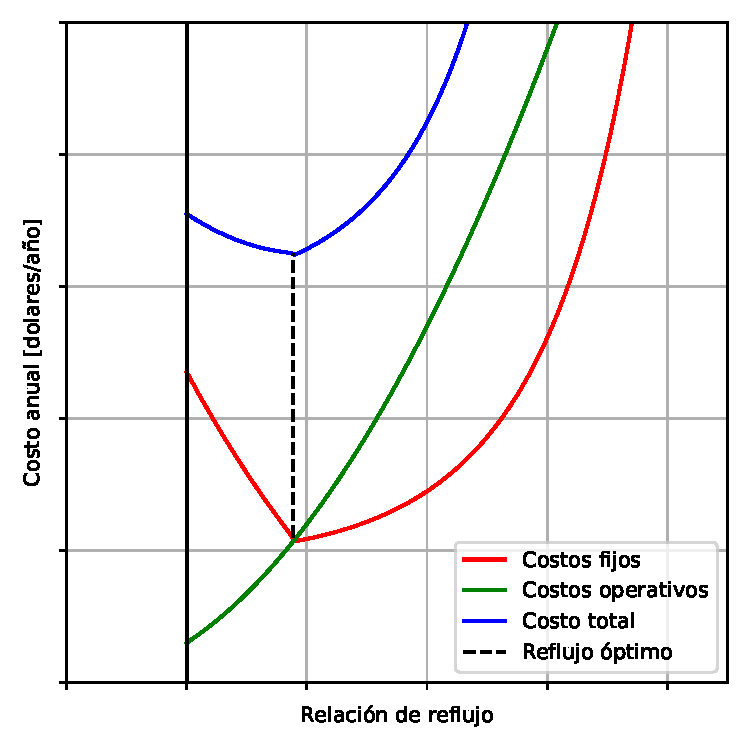
\includegraphics[width=0.4\linewidth]{../resources/images/reflujo_optimo.pdf}
\end{figure}

\begin{itemize}
    \item \textbf{Costos fijos}: No dependen directamente del reflujo y tienden a disminuir a medida que aumenta $R$.
    \item \textbf{Costos de operación}: Dependen del consumo energético y aumentan con $R$, ya que un mayor reflujo requiere más energía en el condensador y el rehervidor.
    \item \textbf{Costo total}: Es la suma de los costos fijos y operativos. Esta curva tiene un punto mínimo.
\end{itemize}

% Jorwin
\newpage
\subsubsection{Condiciones de frontera}
\begin{enumerate}
    \item \textbf{Extremo superior (Condensador total):}\\
          Se asume que todo el vapor que asciende a la parte superior es condensado, de modo que la corriente de vapor saliente es nula. El líquido condensado se divide en dos corrientes: una que se recicla a la columna como reflujo, determinada por la razón de reflujo, y otra que se extrae como destilado. En los balances de masa y energía de esta sección se incorporan estos dos flujos, garantizando la continuidad del reflujo y la extracción del producto.
    \item \textbf{Extremo inferior (rehervidor parcial):}\\
          En la base de la columna se implementa un rehervidor parcial, donde solo se vaporiza una fracción del líquido. Esto establece dos corrientes: una corriente de vapor que asciende en la columna y una corriente líquida que se retira como producto de fondo. El balance de energía en esta zona considera la cantidad de calor suministrado, el cual es suficiente para vaporizar parte del líquido y mantener el equilibrio de fases en la etapa inferior.
    \item \textbf{Condición de alimentación:}\\
          La alimentación se introduce en una etapa intermedia con un flujo y composición determinados, y se asume que se encuentra en estado de saturación (líquido a punto de burbuja) bajo las condiciones operativas de presión. Esta condición fija el punto de inyección y la temperatura de alimentación, que se ajusta mediante el cálculo del punto de burbuja para la composición dada.
\end{enumerate}

Estas condiciones de frontera aseguran que los balances de masa y energía se formulen de manera coherente en los extremos de la columna y en el punto de alimentación, permitiendo la determinación de las variables operativas en estado estacionario.

% Jorwin
\newpage
\subsubsection{Balance de momento}
En una columna de destilación multicomponente con platos perforados (sieve trays), el balance de momento es esencial para garantizar condiciones operativas seguras y evitar dos fenómenos críticos:

\begin{enumerate}
    \item \textbf{Inundación (Flooding):} Fenómeno desencadenado por velocidades de vapor ($u_{j}$) excesivas, donde las fuerzas de arrastre superan la gravedad, transportando líquido a etapas superiores. Este flujo inverso degrada la eficiencia de separación al reducir el tiempo de contacto líquido-vapor, induce perfiles de presión erráticos que distorsionan los cálculos de equilibrio termodinámico ($K_i = f(T_j, P_j)$), y en casos extremos, compromete la integridad mecánica de la columna por sobrecargas estructurales.
    \item \textbf{Goteo (Weeping):} Condición operativa donde velocidades de vapor ($u_{j}$) insuficientes permiten el drenaje no controlado de líquido a través de los orificios del plato. Este flujo descendente evita la formación de la espuma de burbujas necesaria para la transferencia de masa, genera heterogeneidades en la distribución de líquido que desestabilizan los balances de energía, y puede arrastrar componentes pesados al destilado, contaminando productos valiosos.
\end{enumerate}

Es clave considerar las caídas de presión por plato ($\Delta P_{j}$), ya que definen el perfil real de presiones en la columna y evitan errores en el cálculo de las constantes $K_{i}$ (que dependen de $T$ y $P$). Además, $\Delta P_{j}$ está ligada a la velocidad del vapor: valores altos pueden causar inundación y valores bajos favorecen el goteo. Modelar $\Delta P_{j}$ y mantener la velocidad de vapor $u_{j}$ dentro de límites seguros ($u_{\mathrm{min},j} < u_{j} < u_{\mathrm{max},j}$) asegura la estabilidad hidrodinámica necesaria para una operación industrial fiable.

\begin{enumerate}
    \item \textbf{Variables de diseño geométrico:}\\
          Para cada plato se definen las siguientes cantidades, que se emplean en los cálculos de caídas de presión y velocidades:
          $$
              d:\text{ diámetro de cada plato}, \quad
              d_h = a_1\ d:\text{ diámetro de cada hueco}.
          $$
          $$
              A = \pi\ d^2 / 4:\text{ área de cada plato}, \quad
              A_{ac} = a_2\ A:\text{ área activa de cada plato}.
          $$
          $$
              A_{hs}=a_3\ A_{ac}:\text{ área de los huecos}, \quad
              N_{hs}=4\ A_{hs} / \pi\ d_h^{2}:\text{ número de huecos}.
          $$


          donde $a_i$ son fracciones de diseño.
    \item \textbf{Cálculo de densidades por etapa:}\\
          Las densidades de fase líquida $\rho_{L,j}$ y de fase vapor $\rho_{V,j}$ se obtienen a partir de las fracciones molares locales y las propiedades de los componentes presentes. Este cálculo es esencial para determinar con precisión las velocidades y las caídas de presión posteriores.
          \begin{enumerate}
              \item \textbf{Densidad del líquido:}\\
                    Se calcula mediante una media armónica ponderada con base en las densidades puras estimadas y las fracciones molares:
                    $$
                        \rho_{L,j} = \frac{\sum_i x_{i,j} M_{i}}{\sum_i \frac{x_{i,j} M_{i}}{\rho_{L,i}^{\circ}}}
                    $$
              \item \textbf{Densidad del vapor:}\\
                    Asumiendo comportamiento ideal, se utiliza la ley de los gases ideales:
                    $$
                        \rho_{V,j} = \frac{P_j}{R\ T_j}\sum_i y_{i,j} M_i
                    $$

                    donde:
                    \begin{itemize}
                        \item $M_i$: masa molar del componente $i$.
                        \item $\rho_{L,i}^{\circ}$: densidad estandar del componente puro en fase líquida.
                        \item $R$: constante de los gases ideales (8314 J/kmol·K).
                    \end{itemize}
          \end{enumerate}

    \item \textbf{Cálculo de velocidades características:}\\
          La velocidad del vapor en cada etapa $j$ se calcula como:
          $$
              u_j = \frac{\dot{V}_j}{\rho_{V,j}\ A_{ac}}
              \quad\text{con}\quad
              \dot{V}_j = \frac{V_j}{3600}\sum_i y_{i,j} M_i.
          $$

          Las velocidades mínima y máxima se emplean como límites de diseño:
          \begin{enumerate}
              \item \textbf{Velocidad mínima $u_{\min,j}$:}\\
                    Evita el goteo del líquido a través de los huecos.
                    $$
                        u_{\min,j} = k_{\min} \sqrt{\frac{\sigma_j}{\rho_{L,j}\ d_h}}
                    $$
              \item \textbf{Velocidad máxima $u_{\max,j}$:}\\
                    Evita la inundación del plato.
                    $$
                        u_{\max,j} = k_{\max} \sqrt{\frac{\rho_{L,j} - \rho_{V,j}}{\rho_{V,j}}}
                    $$

                    donde $k_{\min}, k_{\max}$ son constantes empíricas.
          \end{enumerate}

    \item \textbf{Cálculo de presión por plato:}\\
          La presión en cada etapa $j$ se determina acumulando las pérdidas desde el condensador. Estas pérdidas de presión $\Delta P_j$ se dividen en tres componentes principales:
          \begin{enumerate}
              \item \textbf{Presión acumulada:}\\
                    $$
                        P_j = P_{\mathrm{condensador}} + \sum_{k=1}^j \Delta P_k
                    $$
              \item \textbf{Caída por fricción del vapor:}\\
                    Basada en una correlación para platos perforados:
                    $$
                        \Delta P_{\mathrm{vap},j} = c_p\ u_j^2\ \rho_{V,j}
                        \quad\text{con}\quad
                        c_p = \frac{1}{334.76\ c_v^2}
                    $$
              \item \textbf{Carga hidrostática del líquido:}\\
                    Asociada a la altura del líquido sobre el plato:
                    $$
                        \Delta P_{\mathrm{liq},j} = \rho_{L,j}\ g\ h_L
                        \quad\text{con}\quad
                        h_L = h_w + h_{ow}
                    $$

                    donde $h_w$ la altura del vertedero y $h_{ow}$ la altura del líquido sobre el vertedero.
              \item \textbf{Efecto capilar:}\\
                    Asociada a la tensión superficial en los huecos del plato:
                    $$
                        \Delta P_{\mathrm{cap},j} = \frac{\sigma_j}{d_h}
                        \left(\frac{\rho_{L,j}}{\rho_{V,j}}\right)^{0.25}
                    $$
              \item \textbf{Suma total de caídas:}
                    $$
                        \Delta P_j = \Delta P_{\mathrm{vap},j}
                        + \Delta P_{\mathrm{liq},j}
                        + \Delta P_{\mathrm{cap},j}
                    $$
          \end{enumerate}

    \item \textbf{Cálculo de la tensión superficial:}\\
          La tensión superficial de una mezcla líquida puede estimarse mediante la correlación de Brock-Bird, que se basa en propiedades críticas y de ebullición estándar. Para una mezcla con fracciones molares $x_i$ a temperatura $T$, la expresión completa es:
          $$
              \sigma = 10^{-3} \left[ 0.1198 \left( 1 + \frac{T_{r,eb}}{1 - T_{r,eb}} \ln(\frac{P_c}{1.013}) \right) - 0.278 \right] \cdot P_c^{2/3} \cdot T_c^{1/3} \cdot (1 - T_r)^{11/9}
          $$

          donde:
          $$
              T_c = \sum_i x_i\ T_{c,i}
              \quad
              P_c = \sum_i x_i\ P_{c,i}
              \quad
              T_{eb} = \sum_i x_i\ T_{eb,i}.
          $$

          y las temperaturas reducidas son:
          $$
              T_r = \frac{T}{T_c},
              \quad
              T_{r,eb} = \frac{T_{eb}}{T_c}.
          $$

    \item \textbf{Cálculo del espaciado entre platos:}\\
          La separación óptima entre platos, $S$, se obtiene imponiendo que la relación característica de operación no supere un valor empírico $k_{\max}$. Esto conduce a la siguiente ecuación en $S$:
          $$
              0.193 \ \biggl(\frac{d_h^2\ \overline{\sigma}}{\overline{\rho}_L}\biggr)^{\!1/8}
              \ \biggl(\frac{\overline{\rho}_L}{\overline{\rho}_V}\biggr)^{\!1/10}
              \ \biggl(\frac{S}{h_L}\biggr)^{\!1/2}
              \;=\; k_{\max},
          $$

          donde ($ \overline{\sigma},\ \overline{\rho}_L,\ \overline{\rho}_V $) son los valores promedio de tensión superficial y densidades de líquido y vapor.
\end{enumerate}

% Jorwin
\newpage
\subsubsection{Preparación de los balances de masa y energía}
Para el desarrollo de los balances de masa y energía que se presentan a continuación, considere el j-ésimo plato de la columna.

\begin{figure}[ht]
    \centering
    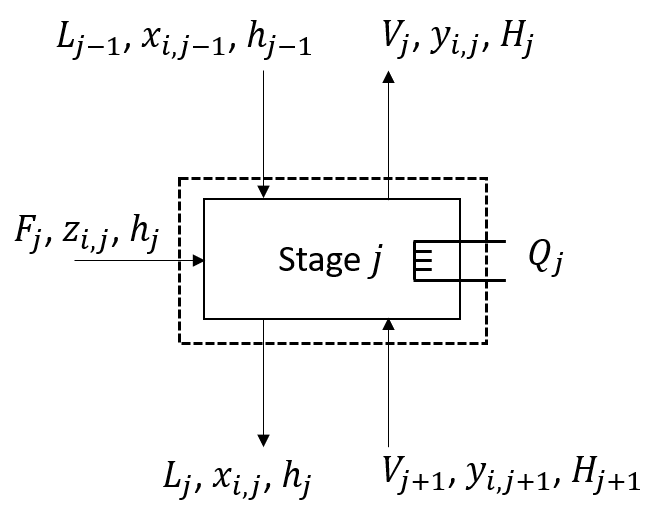
\includegraphics[width=0.5\linewidth]{../resources/flowcharts/balances_plato.png}
    \caption{Diagrama de un plato específico de la columna utilizado para desarrollar los balances de masa y energía.}
\end{figure}

% Jorwin
\subsubsection{Balance de masa}
Dada la naturaleza del problema, se deben formular y resolver numerosos balances de masa en cada etapa de la columna, lo que naturalmente conduce a la generación de un sistema de ecuaciones. Formalmente, para el i-ésimo componente y para el j-ésimo plato se establece un balance de masa de la forma:
$$
    V_{j}\ y_{i,j} + L_{j}\ x_{i,j} - V_{j+1}\ y_{i,j+1} - L_{j-1}\ x_{i,j-1} = F_{j}\ z_{i,j},
$$

donde $V$ y $L$ representan, respectivamente, los flujos molares de vapor y de líquido mientras que F es el flujo de alimentación.

La tasa de flujo líquido $L_k$ se calcula mediante
$$
    L_k = V_{k+1} - D + \sum_{m=0}^{k}F_m
$$

donde $\sum_{m=0}^{k}F_m$ representa la alimentación acumulada hasta la etapa $k$. De este modo, el sistema de ecuaciones resultante depende únicamente de $V_j$ y $V_{j+1}$.

Al recopilar los balances de masa de todas los platos y componentes, se obtiene un sistema de ecuaciones lineales que puede expresarse en forma matricial como:
$$
    A\ x = b,
$$

donde:
\begin{itemize}
    \item $x$ es el vector de incógnitas que representa los caudales molares líquidos del componente en cuestión, es decir, los valores $l_{i,j}$ para cada etapa $j$.
    \item $b$ es el vector de términos constantes que recoge las contribuciones de la alimentación en cada etapa, $F_j z_{i,j}$, así como las condiciones de frontera impuestas en el condensador total y el rehervidor parcial.
    \item $A$ es la matriz de coeficientes, estructurada de forma tridiagonal, que vincula los caudales de vapor y líquido de etapas adyacentes en el balance de masa.
\end{itemize}

Debido a la naturaleza de los balances en la columna, donde cada etapa solo interactúa con las adyacentes (por ejemplo, la etapa $j$ interactúa con $j-1$ y $j+1$), la matriz $A$ presenta una estructura tridiagonal:
$$
    A = \begin{bmatrix}
        b_0    & c_0    & 0      & \cdots  & 0       \\
        a_0    & b_1    & c_1    & \cdots  & 0       \\
        0      & a_1    & b_2    & \cdots  & 0       \\
        \vdots & \vdots & \vdots & \ddots  & c_{n-1} \\
        0      & 0      & 0      & a_{n-1} & b_n
    \end{bmatrix}.
$$

Esta estructura es especialmente ventajosa, ya que permite resolver el sistema de manera muy eficiente utilizando algoritmos específicos para matrices tridiagonales, como el método de Thomas. La formulación en esta forma asegura una solución computacionalmente óptima para el conjunto de balances de masa, facilitando el modelado global de la columna de destilación.

% Edson
\newpage
\subsubsection{Balance de energía}
Las temperaturas en cada plato son necesarias para calcular las entalpías de líquidos y vapores. Formalmente, para el i-ésimo componente y para el j-ésimo plato se establece un balance de energía de la forma:
$$
    V_{j}\ H_j + L_{j}\ h_j - V_{j+1}\ H_{j+1} - L_{j-1}\ h_{j-1} = F_{j}\ h_{F,j} + Q_j
$$

El término $Q_j$ representa la energía retirada o suministrada a las corrientes, para $j=0$ y $j=N$ se estudian los siguientes casos:
\begin{enumerate}
    \item \textbf{Energía retirada en el condensador:}\\
          El condensador es el equipo donde el vapor ascendente proveniente del rehervidor se enfría y condensa, transfiriendo calor al ambiente o a un sistema de enfriamiento \parencite{subsec5_5ref3}.

          La ecuación de balance de energía en el condensador se expresa como:
          $$
              Q_0 = D\ (1 + R)\ (h_0 - H_1)
          $$

          donde:
          \begin{itemize}
              \item $D$ es el flujo molar del destilado.
              \item $R$ es la relación de reflujo.
              \item $h_0$ es la entalpía del líquido en el primer plato.
              \item $H_1$ es la entalpía del vapor en el segundo plato.
          \end{itemize}

    \item \textbf{Energía suministrada en el rehervidor:}\\
          El rehervidor suministra la energía necesaria para vaporizar parte del líquido en el fondo de la columna. Esta energía se aporta generalmente desde una fuente externa, como una caldera. El balance energético considera tanto el calor suministrado como el necesario para mantener la operación del sistema \parencite{subsec5_5ref3}.

          La ecuación de energía en el rehervidor se define como:
          $$
              Q_N = D\ h_0 + B\ h_N - F_{al}\ h_{al} - Q_0
          $$

          donde:
          \begin{itemize}
              \item $D$ es el flujo molar del destilado.
              \item $B$ es el flujo molar del fondo.
              \item $h_N$ es la entalpía del vapor en el último plato.
              \item $F_{al}$ es el flujo molar de la alimentación.
              \item $h_{al}$ es la entalpía de la alimentación en el punto de entrada.
          \end{itemize}
\end{enumerate}

Las entalpías de los vapores y líquidos se calculan a partir de las temperaturas de cada plato:
\begin{enumerate}
    \item \textbf{Entalpía de vapor:}\\
          Se calcula como:
          $$
              H_j = \sum_i y_{ij}\ H^*_i(T_j)
          $$

          donde $H^*_i(T_j)$ es la entalpía del componente $i$ puro.

          Para calcular la entalpía del componente puro, usamos la siguiente ecuación:
          $$
              H^*_i(T_j) = \Delta H^\circ + \int_{T_{\text{ref}, i}}^{T_j} Cp_{V, i}(T)\  dT
          $$

          donde:
          \begin{itemize}
              \item $Cp_{V, i}$ es la capacidad calorífica del vapor.
              \item $\Delta H^\circ$ es la variación de la entalpía a condiciones estándar.
          \end{itemize}

          $Cp_{V, i}$ se calcula utilizando el modelo propuesto en el libro de Termodinámica de \citeauthor{termo_cengel_god}:
          $$
              Cp_{V, i} = A + BT + CT^2 + DT^3
          $$

          Las constantes $A$, $B$, $C$ y $D$ son específicas para cada componente y se obtienen de tablas de propiedades termodinámicas.

    \item \textbf{Entalpía del líquido:}\\
          Se calcula como:
          $$
              h_j = \sum_i x_{ij}\ h^*_i(T_j)
          $$

          donde $h^*_i(T_j)$ es la entalpía del componente $i$ puro.

          Para calcular la entalpía para cada componente puro, se usa la siguiente ecuación:
          $$
              h_{i}(T) = \int_{T_{\text{ref}, i}}^{T_j} Cp_{L, i}(T)\  dT
          $$

          donde $Cp_{L, i}$ es la capacidad calorífica del líquido.

          $Cp_{L, i}$ se calcula utilizando el siguiente modelo:
          $$
              Cp_{V, i} = A + BT + CT^2 + DT^3 + ET^4
          $$

          Las constantes $A$, $B$, $C$ y $D$ son específicas para cada componente y se obtuvieron a partir de datos del $Cp_{L, i}$ a presión estandar y distintas temperaturas, fue necesario hacer regresión para obtener los coeficientes de la ecuación.

    \item \textbf{Entalpía de mezcla de alimentación:}\\
          La entalpía de la mezcla de alimentación se obtiene de la siguiente manera:
          $$
              h = \sum_i z_i\ h^*_i(T_{\text{al}})
          $$

          donde:
          \begin{itemize}
              \item $z_i$ es la fracción molar del componente $i$ en la mezcla de alimentación.
              \item $h^*_i(T_{\text{al}})$ es la entalpía del componente puro $i$ a la temperatura $T_{\text{al}}$, que es la temperatura de la alimentación.
          \end{itemize}

          La entalpía del componente puro se obtiene con la misma integral de entalpía para componente puro en los líquidos.
\end{enumerate}
